%************************************************
% IMPLEMENTATION
%************************************************

\chapter{Implementation} \label{chap: implementation}

\paragraph{} \textit{In this chapter we present the tools that have been used for the implementation of the project, some details about the data, the data preprocessing procedure, a description of the models' configurations and experiments conducted and the produced results.}


%----------------------------------------------------------------
% Tools
%----------------------------------------------------------------

\section{Tools} \label{sec: tools}
\paragraph{} All the computation for this project has been conducted on a university server equipped with Ubuntu SMP version 16.04.1 and a NVIDIA TITAN Xp graphics card for the deep learning training processes. A brief description of the software tools used for the project will follow.

\paragraph{Python} \cite{python} The programming language used for this project is Python v3.6. Python is a general purpose language, known for its ease of use and understanding; however, thanks to the addition of dedicated libraries for data analysis and predictive modeling, in the last few years it has become the reference and most-used language for data science.

\paragraph{Numpy} \cite{numpy} Numpy is an extremely popular and useful library for scientific computing with Python. It allows to easily handle multidimensional data through matrix representation and to perform operation between them thanks to its broadcasting functions. Numpy has been used in all the project implementation's steps to handle and manipulate the data.

\paragraph{Pandas} \cite{pandas} Pandas is an open source library which provides efficient, flexible and easy-to-use data structures and data analysis tools for Python. Pandas is built on top of Numpy library and it is suited to handle almost any kind of data, representing them in a handy tabular form. We mainly used Pandas in order to store the results from the experiments.

\paragraph{matplotlib} \cite{matplotlib} Matplotlib is a 2D plotting library and it represents one of the most common visualization tools for Python. Its \texttt{pyplot} module provides a MATLAB-like functional interface and a wide degree of customization of the generated figures. All the plots in this thesis has been generated using matplotlib library.

\paragraph{scikit-learn} \cite{scikit-learn} Scikit-learn is a well-known, simple and efficient library for data analysis and machine learning in Python. It is open-source and is built on NumPy, SciPy, and matplotlib libraries. It provides several useful tools for data preprocessing, model selection, classification, regression, clustering and dimensionality reduction. In this project, it has been heavily used for the data preprocessing and to implement the classic machine learning models.

\paragraph{XGBoost} \cite{xgboost} XGBoost is an optimized library for distributed gradient boosting, designed to be highly efficient, flexible and portable. It implements a tree-based gradient boosting model which has been used for the gradient boosting experiments.

\paragraph{Tensorflow \& Keras} \cite{tensorflow} \cite{keras} The framework we used in order to build deep learning models is Tensorflow v2.0. Tensorflow is one of the most popular frameworks for machine learning and deep learning; it is open-source and it provides a flexible ecosystem of tools, libraries and community resources to easily build machine learning models. On top of Tensorflow, we used Keras high-level neural networks API. Keras was originally a library separated from Tensorflow, providing ready-to-use tools for fast experimentation and developing of neural networks models by running on top of TensorFlow, CNTK, or Theano. With the update to version 2.0 of Tensorflow, Keras has officially become part of Tensorflow API. We mainly used Keras library on top of Tensorflow for the implementation of deep learning models in order to generate high-level and easy-to-understand code. This choice was reasoned by the fact that this thesis project is also related to the medical field, so we tried to make the code readable also by people which are not specialized in the data scientist field.

\paragraph{Spektral} \cite{Spektral} Spektral is a Python library for graph deep learning, based on the Keras API. It provides a simple but flexible framework for creating graph neural networks (\acsp{gnn}) by making available several ready-to-use, but still highly customizable, graph-based deep learning layers. It also implements functions for the creation of the functional connectivity network from a data stream. In this project, Spektral library was used for the generation of functional connectivity graphs and for the implementation of graph-based deep learning models.


%----------------------------------------------------------------
% Data analysis
%----------------------------------------------------------------

\section{Data analysis} \label{sec: data_analysis}

\paragraph{} For this project, we were provided with 24 hours of \acs{ieeg} data generated from real measurements on a patient suffering form epilepsy. The data contains three seizures, all happening during the first three hours of recording; therefore just the data regarding the first three hours have been used in the project. The brain activity has been measured using 90 electrodes and a sampling frequency of 500 Hz, so each hour contains $1\,800\,000$ time steps of measurements.

First, we identified the position of the seizures in the data and their length. As already mentioned, the data contains three seizures in total, each one having a duration between $13\,000$ and $15\,000$ time steps, for a total of $42\,000$ time steps of seizure. This corresponds to 26 to 30 seconds of duration for each seizure and 84 seconds of seizure in total. Since we had few seizure time steps and the dataset was heavily unbalanced, we had to significantly subsample the data. For this reason, from the beginning of the project we considered only a portion of data around each one of the three seizures, obtaining $450\,000$ time steps (15 minutes) to work with between seizure and non-seizure data in total. This should give an idea of how much limited the amount of useful data was for this project.

Some basic statistical measurements have been applied to the \acs{ieeg} data in order to familiarize with its features. The measured voltage in the \acs{ieeg} vary between about $-9\,500$ and $9\,800$ \acs{uv}, covering a range of about $19\,300$ \acs{uv}. Each electrode's signal oscillates through time with a standard deviation of around 82 \acs{uv} and the various electrodes signals cover different areas of the \acs{ieeg} voltage range based on their placement on the brain surface. In Figure \ref{fig:plot_seizures} the plots of the \acs{ieeg} around the three seizures is shown. The start and end times of the seizures in each plot are indicated by red vertical lines.
\newpage
% \todo{Change following 3 iEEGs to high-quality corresponding images}
% \begin{figure}[H]
%     \centering
%     \begin{subfigure}[t]{0.7\textwidth}
% 		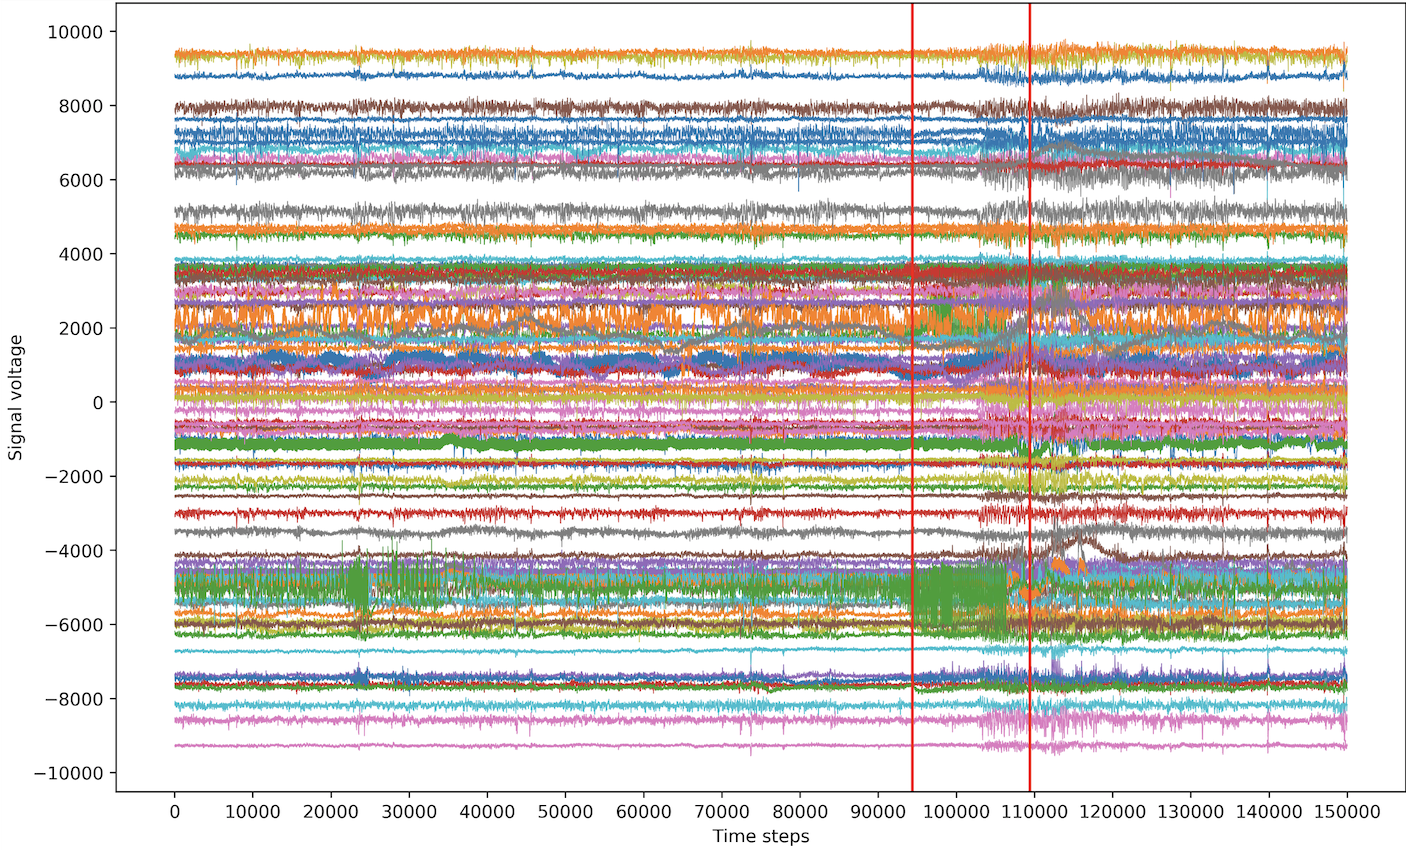
\includegraphics[width=1\textwidth]{plot_seizure1_lowquality}
%         \caption{First epileptic seizure}
%         \label{fig:plot_seizure1}
% 	\end{subfigure}
% 	~
% 	\begin{subfigure}[t]{0.7\textwidth}
% 		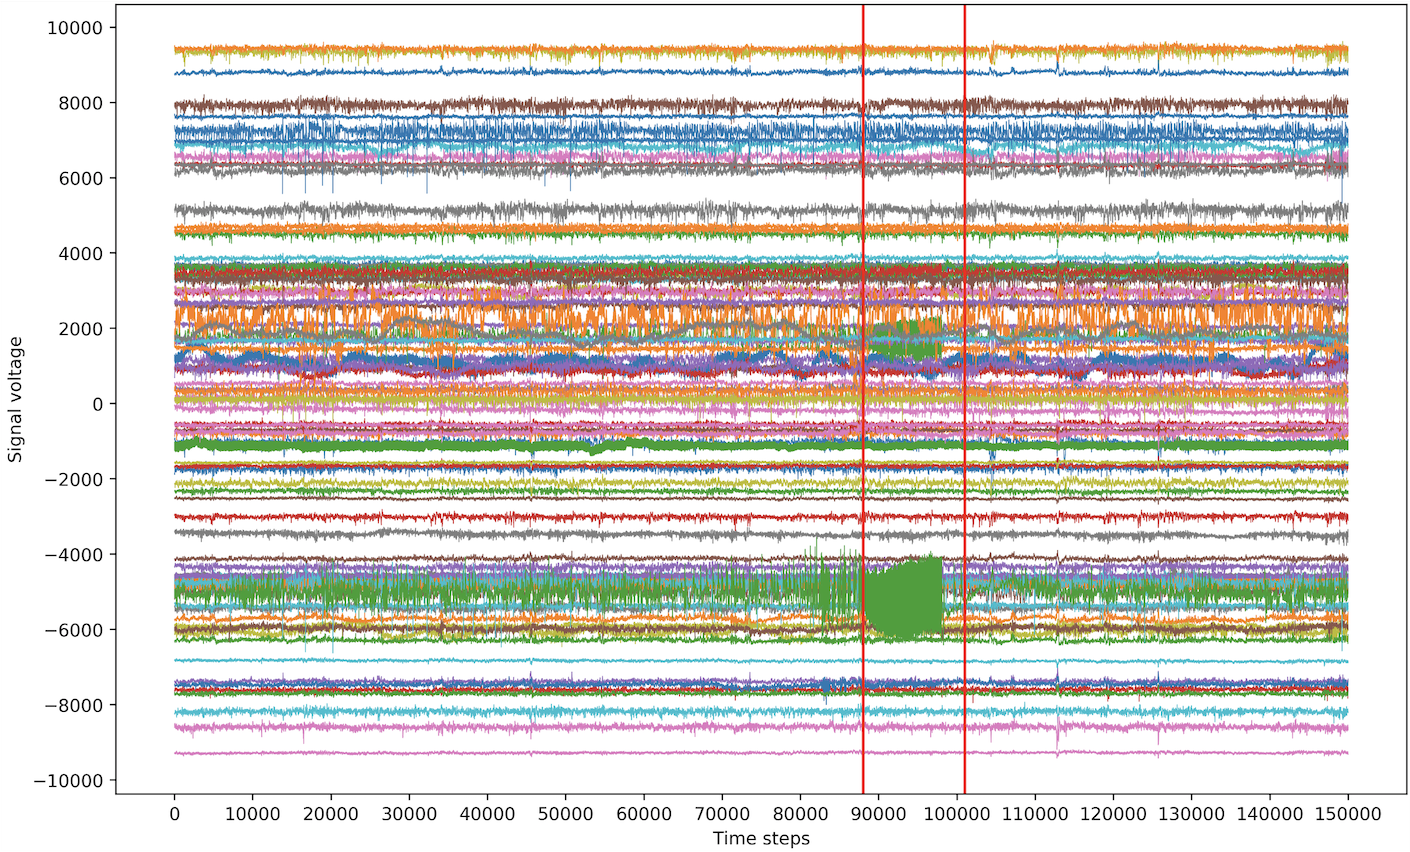
\includegraphics[width=1\textwidth]{plot_seizure2_lowquality}
%         \caption{Second epileptic seizure}
%         \label{fig:plot_seizure2}
%     \end{subfigure}
%     ~
%     \begin{subfigure}[t]{0.7\textwidth}
% 		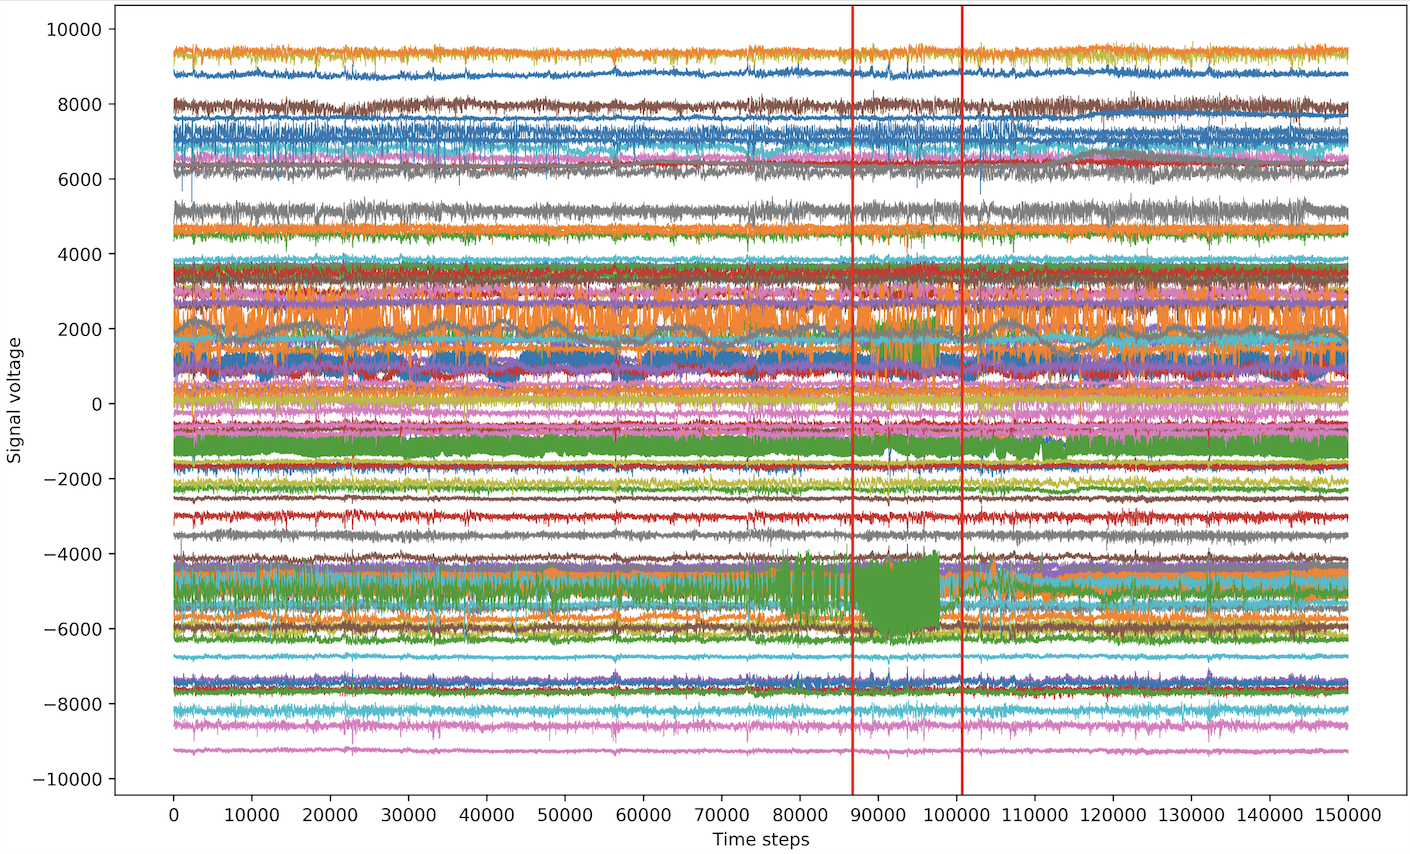
\includegraphics[width=1\textwidth]{plot_seizure3_lowquality}
%         \caption{Third epileptic seizure}
%         \label{fig:plot_seizure3}
% 	\end{subfigure}
%     \caption{Plots of the \acs{ieeg} around the three epileptic seizures (we suggest to zoom-in the figures in the pdf file). The \acs{ieeg} plots show the voltage values of the 90 channels with respect to time, with y axis in common (hence the time-series overlap). The onset and offset of the seizures are marked by red lines.}
%     \label{fig:plot_seizures}
% \end{figure}
\begin{figure}[H]
    \centering
    \begin{subfigure}[t]{0.7\textwidth}
		\includegraphics[width=1\textwidth]{plot_seizure1}
        \caption{First epileptic seizure}
        \label{fig:plot_seizure1}
	\end{subfigure}
	~
	\begin{subfigure}[t]{0.7\textwidth}
		\includegraphics[width=1\textwidth]{plot_seizure2}
        \caption{Second epileptic seizure}
        \label{fig:plot_seizure2}
    \end{subfigure}
    ~
    \begin{subfigure}[t]{0.7\textwidth}
		\includegraphics[width=1\textwidth]{plot_seizure3}
        \caption{Third epileptic seizure}
        \label{fig:plot_seizure3}
	\end{subfigure}
    \caption{Plots of the \acs{ieeg} around the three epileptic seizures (we suggest to zoom-in the figures in the pdf file). The \acs{ieeg} plots show the voltage values of the 90 channels with respect to time, with y axis in common (hence the time-series overlap). The onset and offset of the seizures are marked by red lines.}
    \label{fig:plot_seizures}
\end{figure}
\newpage

Looking at Figure \ref{fig:plot_seizures}, we are not able to precisely identify the presence of a seizure in the \acs{ieeg}, since the task of seizure detection is too complex for an untrained eye and the dynamic of the electrodes signals does not seem to undergo a big change in correspondence of the beginning of a seizure. In any case, we expect the seizure to be represented not directly by the dynamic of the signals, but by the non-linear relations between the electrodes signal's dynamic through time.

The amount of positive time steps, that are the ones inside the seizure portions, corresponds only to the $9.3$\% of the data, with the remaining $90.7$\% of data being negative time steps; therefore we are dealing with very unbalanced data (see Figure \ref{fig:hist_classes}). The extreme unbalance of the data, together with the severe restriction in the amount of data, make this dataset very difficult to work with, but at the same time very similar to a real-world scenario.
\begin{figure}[htbp]
    \centering
    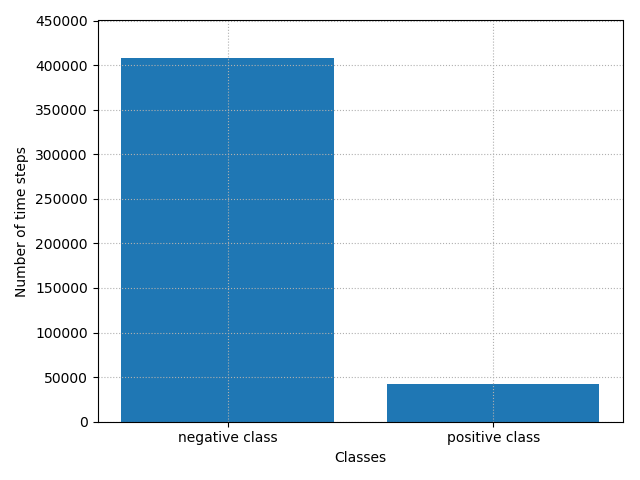
\includegraphics[width=0.6\textwidth]{hist_classes}
    \caption{Histogram of the number of time step for each class}
    \label{fig:hist_classes}
\end{figure}

In order to have an idea of the linear relation between electrodes values, we computed the Pearson correlation coefficient on two sequences of 5 seconds each, one of negative time steps and the other of positive time steps. In Figure \ref{fig:corr_heatmaps} we show the related correlation heatmaps. As you can see from the figures, the correlation heatmap related to the positive time steps reveals a higher linear relation between electrodes values if compared to the correlation heatmap related to the negative time steps. The correlation heatmaps, however, present only the linear relations between data, while we believe that there are hidden non-linear relation between electrodes signal through time which could be crucial for the identification of epileptic seizures.

\begin{figure}[htbp]
    \centering
    \begin{subfigure}[t]{0.49\textwidth}
		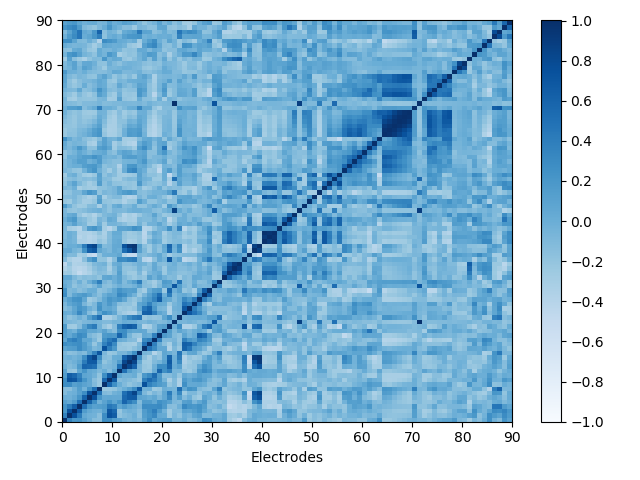
\includegraphics[width=1\textwidth]{corr_nonseizure}
        \caption{Correlation heatmap of 5 seconds of negative time steps}
        \label{fig:corr_nonseizure}
	\end{subfigure}%
	~
	\begin{subfigure}[t]{0.49\textwidth}
		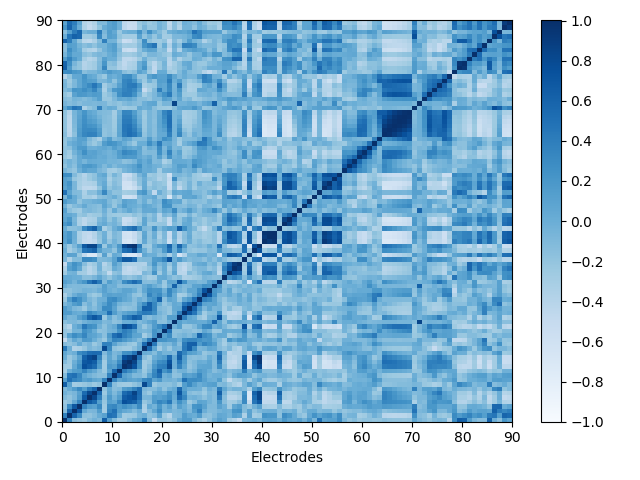
\includegraphics[width=1\textwidth]{corr_seizure}
        \caption{Correlation heatmap of 5 seconds of positive time steps}
        \label{fig:corr_seizure}
    \end{subfigure}
    \caption{Comparison of correlation heatmaps related to negative and positive time steps}
    \label{fig:corr_heatmaps}
\end{figure}

To have another confirmation of the presence of some linear relation between electrodes signals, we computed the standard deviation of the oscillation of each electrode, but this time we computed the mean of the standard deviation both over the negative time steps and over the positive ones. The average standard deviation of the oscillation of each electrode over the negative time steps was around 80 \acs{uv}, while the one over the positive time steps was around 93 \acs{uv}. This shows that, during an epileptic seizure, electrodes signals tends to have wider fluctuation margins, but the difference from the standard fluctuation margins does not seems to be enough to identify a seizure.

%----------------------------------------------------------------
% Data preprocessing
%----------------------------------------------------------------

\section{Data preprocessing} \label{sec: data_preprocessing}
\paragraph{} Once we familiarized with the dataset, we preprocessed it in order to shape it to the right form to be the input of machine learning and deep learning models for the different prediction tasks. As already mentioned in Section \ref{sec: data_analysis_preprocessing}, we divided the data in a training set and a test set, using two seizures' data in the training set and the remaining seizure's data in the test set. The data was prepared to be used by different models for the three prediction tasks described in Section \ref{sec: problem_definition}. Depending on the model and on the task at hand, a sample could represent a time step, a sequence of samples or a sequence of graphs.

\subsection{Time steps as samples}
\paragraph{} This data configuration has been used only for the problem case of detection on a time step; therefore it as been used as input to random forest, gradient boosting, \acs{svm} and dense neural network. In order to prepare data with each time step representing a sample, no additional operations where required, since the dataset was already provided as a big sequence of time step - target couples. Since \acsp{svm} and neural networks are sensible to the scaling of the data, in those cases a \texttt{StandardScaler} from scikit-learn library has been added. The \texttt{StandardScaler} standardize the features of a sample such that the data distribution will have a mean value equal to 0 and a standard deviation value equal to 1. The standardization is computed as:
\begin{align}
    z=\frac{x-\mu}{\sigma} \qquad\qquad \text{with}\qquad &\mu=\frac{1}{N} \sum_{i=1}^{N}\left(x_{i}\right)\\
                                        \text{and}\qquad &\sigma=\sqrt{\frac{1}{N} \sum_{i=1}^{N}\left(x_{i}-\mu\right)^{2}}
\end{align}
where $z$ is the standardized version of $x$, $\mu$ is the mean of $x$ and $\sigma$ is the standard deviation of $x$.

\subsection{Sequences of time steps as samples}
\paragraph{} This data configuration has been used for the problem cases both of detection on a sequence and of prediction on a sequence. The sequences of time steps generated have been the input to standard convolutional and 
\acs{lstm} neural networks. In order to prepare data with each sequence of time steps representing a sample, the dataset has been converted in a set of sequences with a single target associated to each sequence. To do that, we considered different hyperparameters.

The \texttt{'look back'} parameter indicates the number of time steps contained in each sequence; in other words it represents the amount of time steps at which the model can look at in order to predict a target.

The \texttt{'target steps ahead'} parameter determines how far in the future we want the target time step of a sequence to be, starting from the position of the last time step of the sequence. This means that if we consider the \texttt{'target steps ahead'} to be zero, the model will use the sequence's features to predict the target associated with the last time step of the sequence, that corresponds to the problem case of detection on a sequence. Alternatively, if we consider the \texttt{'target steps ahead'} to be higher than zero, the model will use the sequence's features to predict the target associated with a time step outside the sequence and in the future, that corresponds to the problem case of prediction on a sequence.

The \texttt{'stride'} parameter represents the size of the distance between the beginning time step of two consecutive sequences. For instance, if we use a \texttt{'stride'} equal to 1, the sequences will begin time steps at indices $i_0, i_1, i_2, i_3, ...$, while if we use a \texttt{'stride'} equal to 3, the sequences will begin with time steps at indices $i_0, i_3, i_6, i_9, ...$.

The \texttt{'subsampling factor'} parameter allows to downsample the number of sequences by indicating the factor of negative samples to keep with respect to the positive ones. This means that if, for example, we consider the \texttt{'subsampling factor'} to be five, for each positive sample we will keep only five negative samples. This is useful in order to decrease the unbalance in the data. The \texttt{'subsample'} parameter controls whether to apply the downsampling effect or not.

In order to generate the sequences of time steps, we considered one time step index at a time, we took the previous \texttt{'look back'} time steps to create the sequence and we looked \texttt{'target steps ahead'} time steps ahead to identify the target to assign to the sequence. After that, we considered the next time step index, which was \texttt{'stride'} time steps after the current one, and repeated the process. After having created all the sequences, we discarded some random negative sequences in order to respect the proportion between positive and negative samples given by the \texttt{'subsampling factor'}.

In order to create this data configuration, we preprocessed the data by first applying a \texttt{StandardScaler}, like in the previous case, and then generating the sequences both for the training set and the test set, using the same hyperparameters for both of them. The only difference was the fact that we did not use subsampling for the test set, since during the testing of the model we do not need to compensate the unbalance of the dataset.

\subsection{Sequences of graphs as samples}
\paragraph{} This data configuration has been used for the problem cases both of detection on a sequence and of prediction on a sequence. The sequences of graphs generated has been the input to graph-based convolutional and 
\acs{lstm} neural networks. In order to prepare data with each sequence of graphs representing a sample, the first part of the preprocessing process has been the same as for the sequences of time steps: we first applied a \texttt{StandardScaler} and then generated the sequences both for the training set and the test set, without subsampling the test set. After that, an additional operation was required, that is the transformation of the sequences of time steps into sequences of graphs.

As already mentioned in Section \ref{sec: fc_graphs}, the sequences of time steps can be transformed into sequences of graphs by computing the functional connectivity between electrodes and generating a corresponding graph for each time window. To do that, we considered one sequence at a time and we divided it into a fixed number of time windows, each one containing the same number of time steps. For each time window, we built a graph having one node for each electrode and we used the correlation values between electrodes signal in that time window as edge attribute. The number of edges was limited by keeping only the edges with most significative correlation values. Through this process, we generated a graph for each time window in the sequence, therefore the sequence of time steps was transformed in a sequence of graphs. The target remained the same as for sequences of time steps.

This procedure has been implemented with the function \texttt{get\_fc} from \texttt{Spektral} library, which does exactly what just described: it takes a sequence of time steps as input, it divides it in time windows, it computes the functional connectivity between electrodes inside each time window and it outputs the resulting sequence of graphs. For the creation of the sequences of graphs, we considered some additional parameters: the \texttt{'samples per graph'} parameter determines the dimension of the time windows to divide the sequence and the \texttt{'percentiles'} parameter controls which edges in the graphs will be removed. To be more specific, to decide the values for \texttt{'percentiles'}, we choose two numbers between 0 and 100 and we remove from each graph the links with correlation value between the two percentiles.

\subsection{Cross-validation}
\paragraph{} In order to have representative results, we performed k-fold cross validation for all the models and the tasks. Cross validation is a useful technique to evaluate machine learning models, especially when there is a limited amount of data at disposal and we cannot rely on the validation set. In order to perform k-folds cross validation, the dataset is divided into $k$ subsets (folds), of which $k-1$ folds are used as training set and the remaining fold as test set. The training-testing process is performed $k$ times, so that each fold is used as test set one time and it is included in the training set all the other times. To perform cross validation with our data, we divided the dataset into three subsets (3-folds cross validation), each one containing one of the three seizures, and we prepared the three corresponding training and test sets, each time using two folds as training set and the remaining fold as test set.

%----------------------------------------------------------------
% Experiments
%----------------------------------------------------------------

\section{Experiments} \label{sec: experiments}
\paragraph{} As already mentioned in Section \ref{sec: models_application}, a big amount of experiments have been conducted in order to apply the chosen machine learning and deep learning models to the three cases of the problem of epileptic seizures prediction. These experiments helped to identify the best-performing configuration for each model on the task at hand. This section will present the models architectures and parameters that have been tested and the best configuration that has been selected for each model, which generated the results described in section \ref{sec: results}. The best configuration was chosen by looking for the best trade-off between the evaluation metrics over the 3-fold cross-validation.

\subsection{Support Vector Machines experiments}
\paragraph{} The \acs{svm} model has been tested on the problem of detection based on a single time step. We did not make a lot of experiments using \acs{svm}, since the poor results immediately suggested that this machine learning algorithm is too weak to handle the complexity of the seizure prediction task.

In order to test the \acs{svm} model, we used the \texttt{svm.SVC} implementation from scikit-learn library. We kept all the parameters to the default values, except for the \texttt{gamma} and \texttt{class\_weight} parameters. The \acs{svm} has been tested with a penalty parameter $C=1$ and using a Gaussian radial basis function (\acs{rbf}) kernel. The \texttt{gamma} value was set to \texttt{'scale'}, that corresponds to $\frac{1}{F \cdot var(X)}$, where $F$ is the number of features and $var(X)$ is the variance of the input features. We tested both a balanced and an unbalanced version of the \acs{svm} by setting the \texttt{class\_weight} parameter to \texttt{'balanced'} or leaving it to \texttt{None} and we obtained slightly better results using the balanced configuration of the model. Table \ref{tab:svm_param} presents the parameters of the \acs{svm} model that performed better.
\begin{table}[htbp]
    \centering
    \begin{tabular}{ll}
        \hline
        \textbf{Parameter}  & \textbf{Value} \\\hline
        C                   & 1 \\
        kernel              & \texttt{'rbf'} \\
        gamma               & \texttt{'scale'} \\
        balanced            & \texttt{True} \\\hline
    \end{tabular}
    \caption{Parameters of best-performing \acs{svm} model}
    \label{tab:svm_param}
\end{table}

\subsection{Random forests experiments}
\paragraph{} The random forest model has been tested on the problem of detection based on a single time step.

In order to test the random forest model, we used the \texttt{ensemble.RandomForest}-\texttt{Classifier} implementation from scikit-learn library. We kept all the parameters to the default values, except for the \texttt{n\_estimators}, the \texttt{max\_depth} and \texttt{class\_weight} parameters. The \texttt{criterion} parameter to measure the quality of a split was set to \texttt{'gini'}, which corresponds to the Gini impurity function. We tried several values for \texttt{n\_estimators}, which is the number of trees in the forest, and for \texttt{max\_depth}, which is the maximum depth of the tree, in order to find the best balance between the two. We tested both a balanced and an unbalanced version of the random forest classifier by setting the \texttt{class\_weight} parameter to \texttt{'balanced'} or leaving it to \texttt{None} and there was no resulting difference between the two configurations. Table \ref{tab:randomforest_param} presents the parameters of the random forest model that performed better.
\begin{table}[htbp]
    \centering
    \begin{tabular}{ll}
        \hline
        \textbf{Parameter}  & \textbf{Value} \\\hline
        n\_estimators       & 20 \\
        max\_depth          & 8 \\
        criterion           & \texttt{'gini'} \\
        balanced            & \texttt{True/False} \\\hline
    \end{tabular}
    \caption{Parameters of best-performing random forest model}
    \label{tab:randomforest_param}
\end{table}

\subsection{Gradient boosting experiments}
\paragraph{} The gradient boosting model has been tested on the problem of detection based on a single time step.

In order to test the gradient boosting model, we used the \texttt{XGBClassifier} implementation from xgboost library. We kept all the parameters to the default values, except for the \texttt{n\_estimators}, the \texttt{max\_depth} and \texttt{scale\_pos\_weight} parameters. The \texttt{booster} parameter was set to \texttt{'gbtree'} in order to use a tree-based booster. As for the random forest model, we tried different values for \texttt{n\_estimators} and for \texttt{max\_depth} in order to find the best balance between the two. We tested both a balanced and an unbalanced version of the random forest classifier by setting the \texttt{scale\_pos\_weight} parameter to $\frac{\texttt{num\_negative}}{\texttt{num\_positive}}$, which are respectively the number of negative and positive samples, or by leaving it to \texttt{None} and there was no resulting difference between the two configurations. Table \ref{tab:gradientboosting_param} presents the parameters of the gradient boosting model that performed better.
\begin{table}[htbp]
    \centering
    \begin{tabular}{ll}
        \hline
        \textbf{Parameter}  & \textbf{Value} \\\hline
        n\_estimators       & 20 \\
        max\_depth          & 4 \\
        booster             & \texttt{'gbtree'} \\
        balanced            & \texttt{True/False} \\\hline
    \end{tabular}
    \caption{Parameters of best-performing gradient boosting model}
    \label{tab:gradientboosting_param}
\end{table}

\subsection{Dense neural networks experiments}
\paragraph{} The dense neural network model has been tested on the problem of detection based on a single time step.

In order to test the \acs{fcnn} model, we used the \texttt{Dense} and \texttt{Dropout} layers implementation from Tensorflow's Keras library. We investigated several configurations of the model by trying different values for the number of dense layers (\texttt{depth\_dense}), the number of units in each layer (\texttt{units}), the activation function to use (\texttt{activation}), the amount of $\ell_2$ regularization to apply to the kernel (\texttt{kernel\_regularizer}) and the dropout rate to apply between the dense layers (\texttt{dropout}). During the training of the model, we used the \texttt{class\_weight} parameter to compensate the unbalance of the dataset.

The model configuration which obtained the best results is composed by three fully-connected layers, with a dropout layer after each one of them. The first two dense layer have 512 units, while the third one has 256 units, and they all use the \acs{relu} activation function and the $\ell_2$ kernel regularization. After the three dense layers, there is a fourth dense layer with only 1 unit and a sigmoid activation function in order to output the prediction. Table \ref{tab:dense_param} presents the parameters of the dense neural network model that performed better.
\begin{table}[htbp]
    \centering
    \begin{tabular}{ll}
        \hline
        \textbf{Parameter}  & \textbf{Value} \\\hline
        epochs              & 20 \\
        batch\_size         & 32 \\
        depth\_dense        & 4 \\
        units               & 512 / 256 \\
        activation          & \texttt{'relu'} \\
        kernel\_regularizer & \texttt{l2(5e-2)} \\
        dropout             & 0.4 \\
        class\_weight       & \{0: $\frac{N}{\texttt{num\_negative}}$, 1: $\frac{N}{\texttt{num\_positive}}$\} \\\hline
    \end{tabular}
    \caption{Parameters of best-performing dense neural network model}
    \label{tab:dense_param}
\end{table}

\subsection{Convolutional neural networks experiments}
\paragraph{} The convolutional neural network model has been tested on the problems of detection and prediction based on a sequence of time steps.

In order to test the \acs{cnn} model, we used the \texttt{Conv1D}, \texttt{MaxPooling1D}, \texttt{Flatten}, \texttt{Dense}, \texttt{Dropout} and \texttt{BatchNormalization} layers implementation from Tensorflow's Keras library. We investigated several configurations of the model by first trying different values for the main parameters of the neural network: the number of convolutional layers (\texttt{depth\_conv}), the number of dense layers for the prediction (\texttt{depth\_dense}), the number of output filters in the convolution (\texttt{filters}), the length of the convolution window (\texttt{kernel\_size}), the activation function to use (\texttt{activation}), the amount of $\ell_2$ regularization to apply to the kernel (\texttt{kernel\_regularizer}), the presence of batch normalization (\texttt{batch\_norm}) and the dropout rate (\texttt{dropout}) to apply between the dense layers. During the training of the model, we used the \texttt{class\_weight} parameter to compensate the unbalance of the dataset.

After the first promising results, we tried to improve the performances of the model by using dilated convolution. Using this technique, the filter is "dilated" before its application, meaning that its size is expanded by filling the empty positions with zeros. This means that the filter's dimensions are not altered, but its weights are matched to not-adjacent instances in the input matrix. The distance between the instances is determined by the dilation rate $D$. Figure \ref{fig:nn_conv_dilated} shows an example of a $3 \times 3$ dilated convolution with $D=2$.
\begin{figure}[htbp]
    \centering
    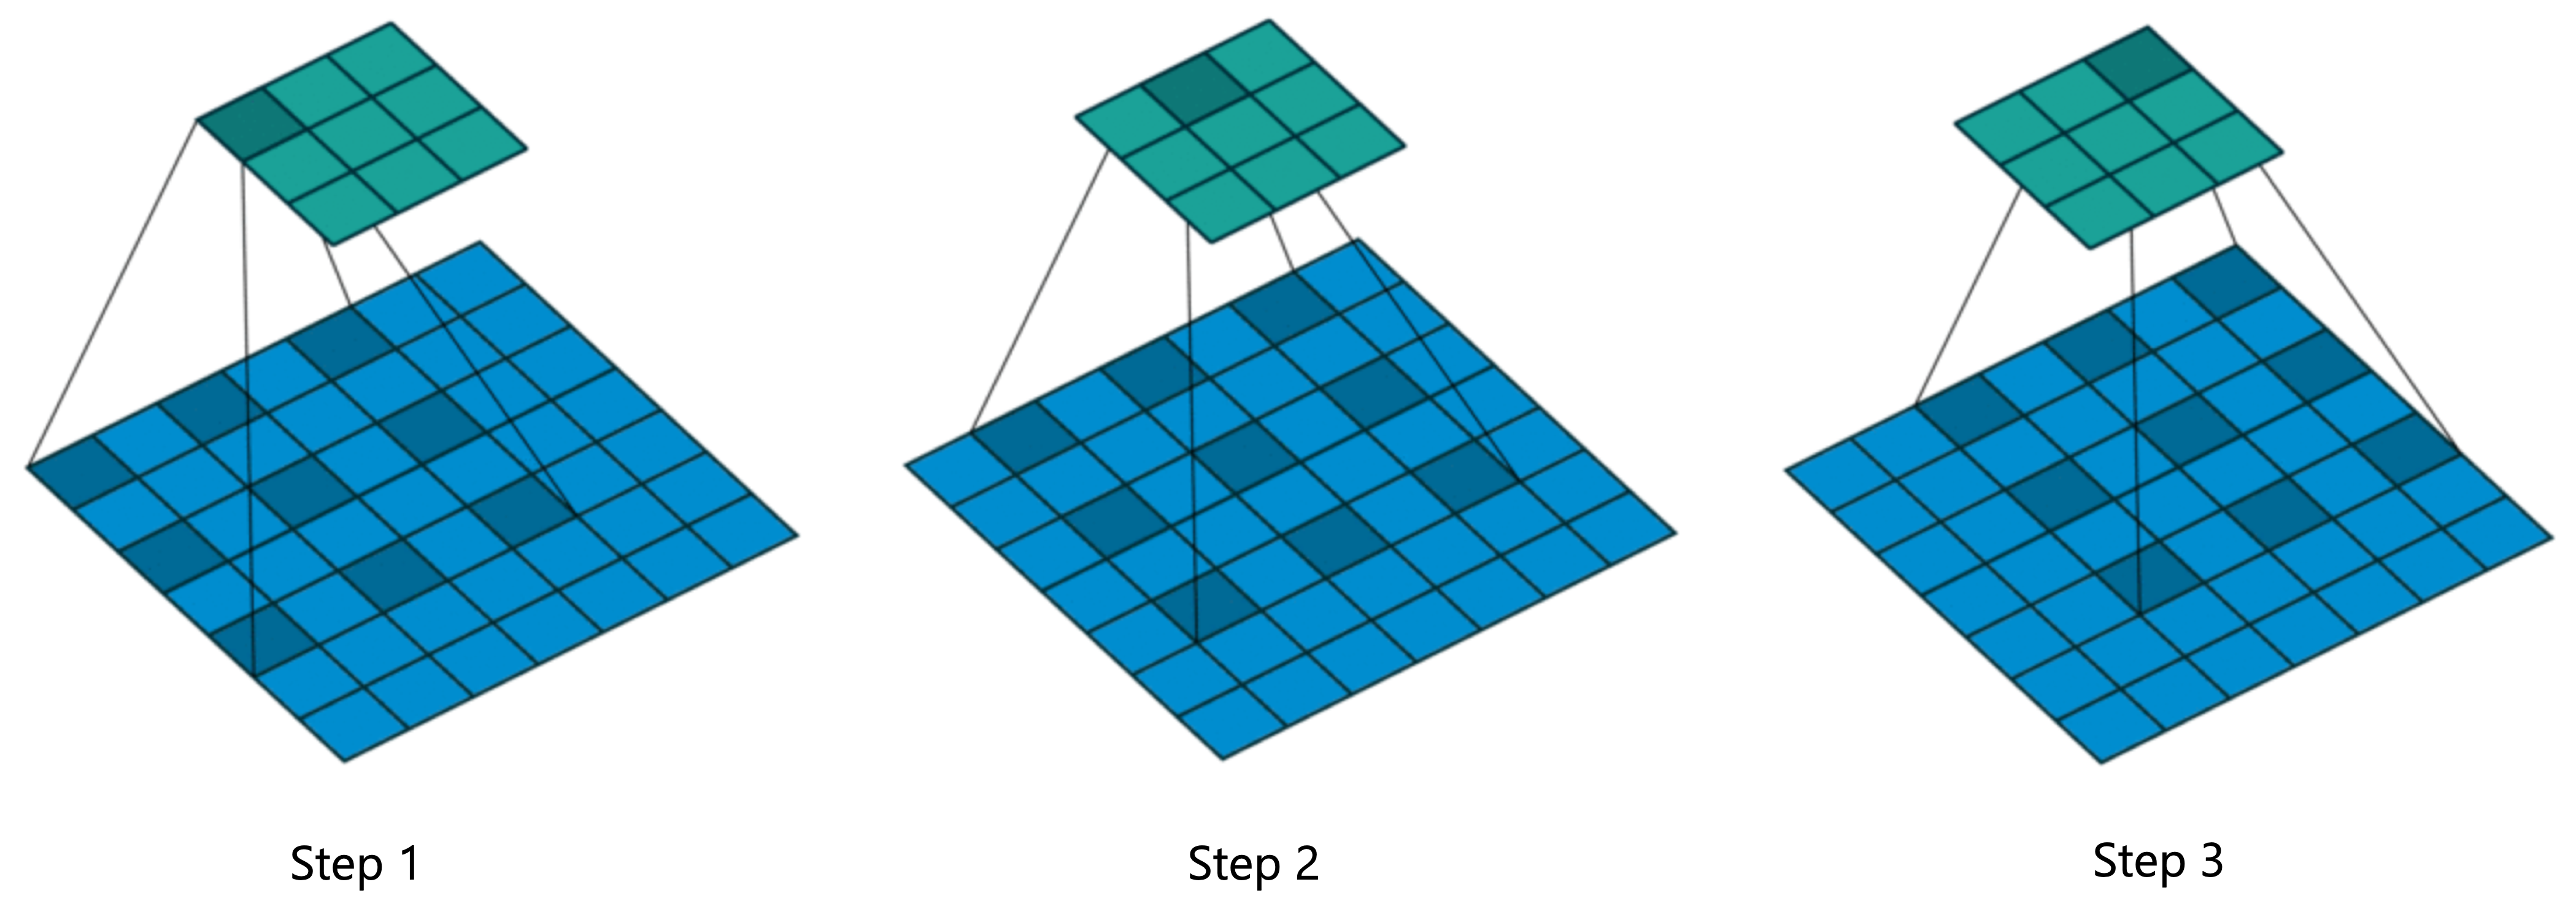
\includegraphics[width=0.8\textwidth]{nn_conv_dilated}
    \caption{Sequence of receptive fields with dilation rate equal to 2 (from \textit{Medium - Towards Data Science})}
    \label{fig:nn_conv_dilated}
\end{figure}

In order to test the model with dilated convolution, we added the dilation rate (\texttt{dilation\_rate}) parameter to the hyperparameters search and we set the padding (\texttt{padding}) to \texttt{'causal'}. In this way, we are limiting the filter at time step $t$ so that it can only see inputs that are no later than $t$. This is done by padding the layer's input with zeros in the front. In order to generalize better, we also added a max-pooling layer after each convolutional layer (\texttt{pooling}).

The \acs{cnn} model was tested both on detection and prediction problems and on different values of \texttt{look\_back} and \texttt{target\_steps\_ahead} for the creation of the input sequences, so we identified different "best" configurations. In general, the architecture that worked better is composed by two or three convolutional layers, each one followed by a max-pooling layer, and by two final fully-connected layers (the first one having 256 units), with a batch normalization layer and a dropout layer between the two. The convolutional layers use 64 filters, except for the last one which uses 32 filters; the kernel size is set to 3 and the convolution is made with a dilation rate equal to 3. All the layers use the \acs{relu} activation function and the $\ell_2$ kernel regularization, except for the last dense layer, which has only 1 unit and which uses a sigmoid activation function in order to output the prediction. 

Table \ref{tab:conv_param} presents the parameters of the dense neural network model that performed better. The best-performing parameters are the same both for the detection and prediction problems, with the only difference in the number of convolutional layers, which for the prediction task varies between two and three depending on the value of \texttt{target\_steps\_ahead}.
\begin{table}[htbp]
    \centering
    \begin{tabular}{ll}
        \hline
        \textbf{Parameter}  & \textbf{Value} \\\hline
        epochs              & 10 \\
        batch\_size         & 64 \\
        depth\_conv         & 2 \\
        depth\_dense        & 2 \\
        filters             & 64 \\
        kernel\_size        & 3 \\
        activation          & \texttt{'relu'} \\
        batch\_norm         & \texttt{True} \\
        kernel\_regularizer & \texttt{l2(5e-1)} \\
        dropout             & 0.4 \\
        pooling             & \texttt{True} \\
        pool\_size          & 2 \\
        padding             & \texttt{'causal'} \\
        dilation\_rate      & 3 \\
        class\_weight       & \{0: $\frac{N}{\texttt{num\_negative}}$, 1: $\frac{N}{\texttt{num\_positive}}$\} \\\hline
    \end{tabular}
    \caption{Parameters of best-performing convolutional neural network model}
    \label{tab:conv_param}
\end{table}

\subsection{\acs{lstm} neural networks experiments}
\paragraph{} The \acs{lstm} neural network model has been tested on the problems of detection and prediction based on a sequence of time steps.

In order to test the \acs{lstm} model, we used the \texttt{LSTM}, \texttt{Dense}, \texttt{Dropout} and \texttt{Batch}-\texttt{Normalization} layers implementation from Tensorflow's Keras library. We investigated several configurations of the model by trying different values for the number of \acs{lstm} layers (\texttt{depth\_lstm}), the number of dense layers (\texttt{depth\_dense}), the number of units in each \acs{lstm} layer (\texttt{units\_lstm}), the activation function to use (\texttt{activation}), the amount of $\ell_2$ regularization to apply to the kernel (\texttt{kernel\_regularizer}), the presence of batch normalization (\texttt{batch\_norm}) and the dropout rate (\texttt{dropout}) to apply between the layers. During the training of the model, we used the \texttt{class\_weight} parameter to compensate the unbalance of the dataset.

The \acs{lstm} model was tested both on detection and prediction problems and on different values of \texttt{look\_back} and \texttt{target\_steps\_ahead} for the creation of the input sequences; however we identified a single configuration that obtained the best results in all the tasks. The architecture that worked better is composed by one \acs{lstm} layer followed by two fully-connected layers (the first one having 256 units), with a batch normalization layer and a dropout layer between the three layers. The \acs{lstm} layer uses 256 units and all the layers use the \acs{relu} activation function and the $\ell_2$ kernel regularization, except for the last dense layer, which has only 1 unit and which uses a sigmoid activation function in order to output the prediction. Table \ref{tab:lstm_param} presents the parameters of the \acs{lstm} neural network model that performed better.
\begin{table}[htbp]
    \centering
    \begin{tabular}{ll}
        \hline
        \textbf{Parameter}  & \textbf{Value} \\\hline
        epochs              & 15 \\
        batch\_size         & 64 \\
        depth\_lstm         & 1 \\
        depth\_dense        & 2 \\
        units\_lstm         & 256 \\
        activation          & \texttt{'relu'} \\
        batch\_norm         & \texttt{True} \\
        kernel\_regularizer & \texttt{l2(5e-1)} \\
        dropout             & 0.4 \\
        class\_weight       & \{0: $\frac{N}{\texttt{num\_negative}}$, 1: $\frac{N}{\texttt{num\_positive}}$\} \\\hline
    \end{tabular}
    \caption{Parameters of best-performing \acs{lstm} neural network model}
    \label{tab:lstm_param}
\end{table}

\subsection{Graph-based convolutional neural networks experiments}
\paragraph{} The graph-based convolutional neural network model has been tested on the problems of detection and prediction based on a sequence of graphs.

The graph-based \acs{cnn} model has been implemented and tested in the same way as the standard \acs{cnn} model, conducting hyperparameters search on the same parameters and using a similar architecture. The main difference is the addition of an edge-conditioned convolutional layer (\acs{ecc}), followed by a global average-pooling, just before the use of the standard \acs{cnn}. This is necessary in order to convert the input graphs into expressive features that can be processed by the standard \acs{cnn}. In addition to the \acs{cnn} parameters, we tested different values also for the number of output filters in the edge-conditioned convolution (\texttt{g\_filters}).

The graph-based \acs{cnn} model was tested both on detection and prediction problems and on different values of \texttt{look\_back} and \texttt{target\_steps\_ahead} for the creation of the input sequences; however we identified a single configuration that obtained the best results in all the tasks, even though the graph-based \acs{cnn} performance in general were poor. As already mentioned, the configuration is the same as for the standard \acs{cnn} with a \acs{ecc} and a global average-pooling layers added at the beginning. Table \ref{tab:gconv_param} presents the parameters of the graph-based convolutional neural network model that performed better.
\begin{table}[htbp]
    \centering
    \begin{tabular}{ll}
        \hline
        \textbf{Parameter}  & \textbf{Value} \\\hline
        epochs              & 200 \\
        batch\_size         & 32 \\
        depth\_conv         & 3 \\
        depth\_dense        & 2 \\
        filters             & 64 \\
        kernel\_size        & 3 \\
        g\_filters          & 32 \\
        activation          & \texttt{'relu'} \\
        batch\_norm         & \texttt{True} \\
        kernel\_regularizer & \texttt{l2(5e-3)} \\
        dropout             & 0.4 \\
        pooling             & \texttt{True} \\
        pool\_size          & 2 \\
        padding             & \texttt{'causal'} \\
        dilation\_rate      & 3 \\
        class\_weight       & \{0: $\frac{N}{\texttt{num\_negative}}$, 1: $\frac{N}{\texttt{num\_positive}}$\} \\\hline
    \end{tabular}
    \caption{Parameters of best-performing graph-based convolutional neural network model}
    \label{tab:gconv_param}
\end{table}

\subsection{Graph-based \acs{lstm} neural networks experiments}
\paragraph{} The graph-based \acs{lstm} neural network model has been tested on the problems of detection and prediction based on a sequence of graphs.

The graph-based \acs{lstm} model has been implemented and tested in the same way as the standard \acs{lstm} model, conducting hyperparameters search on the same parameters and using a similar architecture. The main difference is the addition of an edge-conditioned convolutional layer (\acs{ecc}), followed by a global average-pooling, just before the use of the standard \acs{lstm}. This is necessary in order to convert the input graphs into expressive features that can be processed by the standard \acs{lstm}. In addition to the \acs{lstm} parameters, we tested different values also for the number of output filters in the edge-conditioned convolution (\texttt{g\_filters}).

The graph-based \acs{lstm} model was tested both on detection and prediction problems and on different values of \texttt{look\_back} and \texttt{target\_steps\_ahead} for the creation of the input sequences; however we identified a single configuration that obtained the best results in all the tasks, even though the graph-based \acs{lstm} performance in general were poor. As already mentioned, the configuration is the same as for the standard \acs{lstm} with a \acs{ecc} and a global average-pooling layers added at the beginning. Table \ref{tab:glstm_param} presents the parameters of the graph-based \acs{lstm} neural network model that performed better.
\begin{table}[htbp]
    \centering
    \begin{tabular}{ll}
        \hline
        \textbf{Parameter}  & \textbf{Value} \\\hline
        epochs              & 150 \\
        batch\_size         & 32 \\
        depth\_lstm         & 1 \\
        depth\_dense        & 2 \\
        units\_lstm         & 256 \\
        g\_filters          & 32 \\
        activation          & \texttt{'relu'} \\
        batch\_norm         & \texttt{True} \\
        kernel\_regularizer & \texttt{l2(5e-3)} \\
        dropout             & 0.4 \\
        class\_weight       & \{0: $\frac{N}{\texttt{num\_negative}}$, 1: $\frac{N}{\texttt{num\_positive}}$\} \\\hline
    \end{tabular}
    \caption{Parameters of best-performing graph-based \acs{lstm} neural network model}
    \label{tab:glstm_param}
\end{table}


%----------------------------------------------------------------
% Results evaluation
%----------------------------------------------------------------

\section{Results evaluation} \label{sec: results}
\paragraph{} For the models evaluation, as already mentioned, four metrics have been used: loss, accuracy, ROC-AUC and recall. In order to evaluate models, we chose as best models the ones that obtained highest recall on test data. For this type of task, recall is very important, as it represents the number of true positive instances ($TP$) over the total number of real positive instances ($TP+FN$); therefore it is able to tell us the probability of correct prediction of a seizure. Being totally focused on the positive class, recall is an evaluation metric particularly suited to unbalanced datasets, since it is not influenced by the number of negative instances. Also ROC-AUC had a crucial role in models evaluation, since we want the classifiers to be consistent and to avoid random prediction. Of course, loss and accuracy have not been ignored, since the models need to correctly classify more than the majority of time steps in order to be significant.

To sum up, in order to choose the preferred configuration for the models, we looked for the best trade-off between the four metrics, slightly prioritizing recall over the others. Following this logic, we selected the best model for each machine learning and deep learning method used on each type of task. This allowed us to make a comparison between the performances of different methods for each task.

As already mentioned before, all the results presented have been computed by taking the mean over the 3-fold cross-validation. When choosing the best models, we payed attention also to the standard deviation of the recall over the three folds, in order to avoid choosing a model that can perform extraordinarily well on a fold and awfully on another fold.


\subsection{Detection on a time step}
\paragraph{} The results of \acs{svm}, random forest, gradient boosting and \acs{fcnn} models on the problem of seizure detection based on a single time step are presented in Table \ref{tab:det_timestep_results} and shown as a barplot in Figure \ref{fig:det_timestep_plots}.
\begin{table}[b]
    \centering
    \begin{tabular}{lllll}
        \hline
                          & \multicolumn{4}{c}{\textbf{Metric}}                                    \\ \cline{2-5} 
        \textbf{Model}    & \textit{loss} & \textit{accuracy} & \textit{ROC-AUC} & \textit{recall} \\ \hline
        SVM               & 2.497         & 75.1 \%           & 0.601            & 0.067           \\
        random forest     & 0.303         & 89.9 \%           & 0.768            & 0.121           \\
        gradient boosting & 0.297         & 89.8 \%           & 0.805            & 0.219           \\
        FCNN              & 0.293         & 90.2 \%           & 0.734            & \textbf{0.248}  \\\hline
    \end{tabular}
    \caption{Results of the models for the problem of detection on a time step}
    \label{tab:det_timestep_results}
\end{table}

\begin{figure}[t]
    \centering
    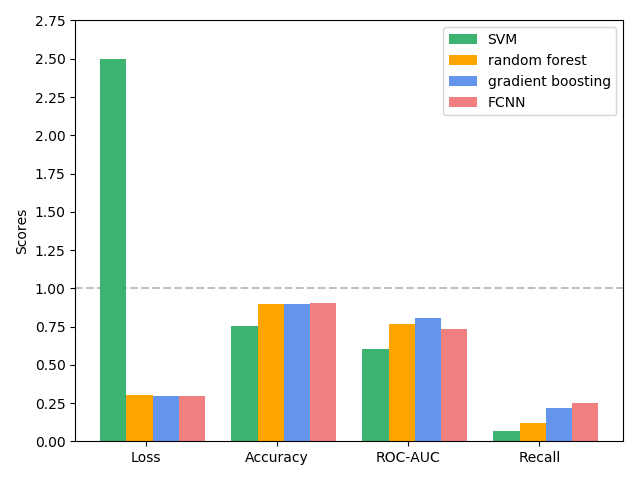
\includegraphics[width=0.7\textwidth]{det_timestep_plots}
    \caption{Barplot of results of the models for the problem of detection on a time step}
    \label{fig:det_timestep_plots}
\end{figure}

As expected, the results on this type of problem were unsatisfactory, since the values of recall do not even come close to the half of positive instances. This means that most of the times the models are not able to correctly detect the presence of a seizure only looking at the features of a single time step. Except for the \acs{svm} model, which obtained the worst results, the other models obtained acceptable performances in predicting general instances, since the accuracy values are around 90 \% and, looking at the ROC-AUC values, the predictions are not random.

The model that performed better on this task was the dense neural network, which was able to correctly detect about a quarter of the positive samples.


\subsection{Detection on a sequence}
\paragraph{} The results of \acs{cnn}, \acs{lstm}, graph-based \acs{cnn} and graph-based \acs{lstm} models on the problem of seizure detection based on a sequence are presented in Table \ref{tab:det_sequence_results} and shown as a barplot in Figure \ref{fig:det_sequence_plots}.
\begin{table}[t]
    \centering
    \begin{tabular}{lllll}
        \hline
                          & \multicolumn{4}{c}{\textbf{Metric}}                                    \\ \cline{2-5} 
        \textbf{Model}    & \textit{loss} & \textit{accuracy} & \textit{ROC-AUC} & \textit{recall} \\ \hline
        CNN               & 0.208         & 94.2 \%           & 0.903            & 0.534           \\
        LSTM              & 0.221         & 95.3 \%           & 0.910            & \textbf{0.580}  \\
        graph-based CNN   & 2.268         & 29.7 \%           & 0.667            & 0.895           \\
        graph-based LSTM  & 1.484         & 69.2 \%           & 0.616            & 0.476           \\\hline
    \end{tabular}
    \caption{Results of the models for the problem of detection on a sequence}
    \label{tab:det_sequence_results}
\end{table}

\begin{figure}[t]
    \centering
    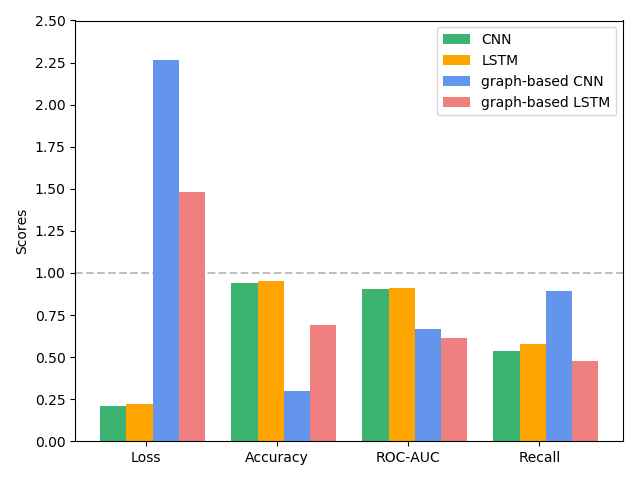
\includegraphics[width=0.7\textwidth]{det_sequence_plots}
    \caption{Barplot of results of the models for the problem of detection on a sequence}
    \label{fig:det_sequence_plots}
\end{figure}

For this type of task, tested different values of \texttt{'look back'} and chose the one that worked better for each model: the CNN model looked at sequences of 100 time steps each; the LSTM model looked at sequences of 200 time steps each; both the graph-based models looked at sequences of 5000 time steps each, corresponding to 10 graphs, each one representing a window of 500 time steps.

The standard \acs{cnn} and \acs{lstm} models achieved acceptable performances, being able to correctly detect more than half of the positive samples. They obtained similar results, but the \acs{lstm} was the model that performed better, since it was able to obtain an higher recall with respect to the \acs{cnn} model. On the other hand, the graph-based models performed very poorly, reaching high loss values, and their prediction where not so far from random predictions. The high recall obtained by the graph-based \acs{cnn} model could be misleading, but the values of the other metrics suggest that it is due to the fact that the model predicts 1 most of the times, without really being able to detect a seizure.


\subsection{Prediction on a sequence}
\paragraph{} For this type of task, after several experiments, we came to the conclusion that the models were not able to correctly predict targets more than 2000 time steps (4 seconds) forward. Passed that threshold, their performances started to rapidly degenerate. For this reason, we chose three \texttt{'target steps ahead'} values as reference for the models evaluation: 500 time steps (1 second), 1000 time steps (2 seconds) and 2000 time steps (4 seconds) forward. The results of \acs{cnn}, \acs{lstm}, graph-based \acs{cnn} and graph-based \acs{lstm} models on the problem of seizure prediction based on a sequence are presented in different tables and barplots based on the value of \texttt{'target steps ahead'}.

Table \ref{tab:pred_sequence500_results} and the barplot in Figure \ref{fig:pred_sequence500_plots} show the results for the prediction of a target 500 time steps (1 second) forward with respect to the associated sequence.
\begin{table}[htbp]
    \centering
    \begin{tabular}{lllll}
        \hline
                          & \multicolumn{4}{c}{\textbf{Metric}}                                    \\ \cline{2-5} 
        \textbf{Model}    & \textit{loss} & \textit{accuracy} & \textit{ROC-AUC} & \textit{recall} \\ \hline
        CNN               & 0.340         & 89.2 \%           & 0.946            & 0.634           \\
        LSTM              & 0.293         & 92.2 \%           & 0.922            & \textbf{0.708}  \\
        graph-based CNN   & 1.812         & 29.1 \%           & 0.570            & 0.877           \\
        graph-based LSTM  & 1.532         & 67.4 \%           & 0.558            & 0.377           \\\hline
    \end{tabular}
    \caption{Results of the models for the problem of prediction on a sequence with the target 500 time steps (1 second) forward}
    \label{tab:pred_sequence500_results}
\end{table}

\begin{figure}[htbp]
    \centering
    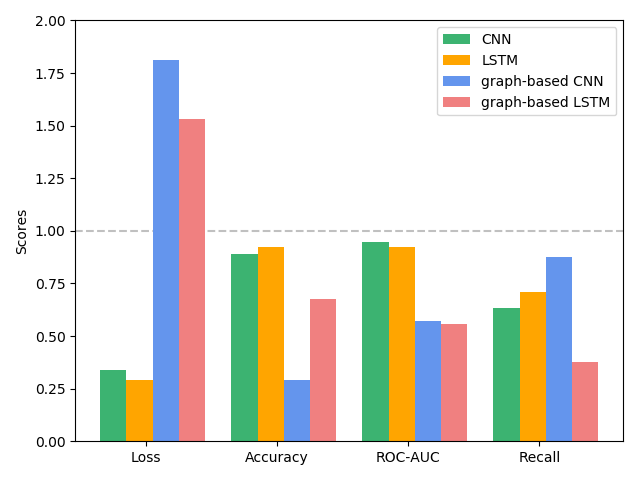
\includegraphics[width=0.7\textwidth]{pred_sequence500_plots}
    \caption{Barplot of results of the models for the problem of prediction on a sequence with the target 500 time steps (1 second) forward}
    \label{fig:pred_sequence500_plots}
\end{figure}

For this configuration, the CNN model looked at sequences of 500 time steps each; the LSTM model looked at sequences of 200 time steps each; both the graph-based models looked at sequences of 5000 time steps each, corresponding to 10 graphs, each one representing a window of 500 time steps.

Table \ref{tab:pred_sequence1000_results} and the barplot in Figure \ref{fig:pred_sequence1000_plots} show the results for the prediction of a target 1000 time steps (2 seconds) forward with respect to the associated sequence.
\begin{table}[htbp]
    \centering
    \begin{tabular}{lllll}
        \hline
                          & \multicolumn{4}{c}{\textbf{Metric}}                                    \\ \cline{2-5} 
        \textbf{Model}    & \textit{loss} & \textit{accuracy} & \textit{ROC-AUC} & \textit{recall} \\ \hline
        CNN               & 0.224         & 92.4 \%           & 0.930            & \textbf{0.702}  \\
        LSTM              & 0.180         & 95.4 \%           & 0.908            & 0.637           \\
        graph-based CNN   & 2.990         & 32.9 \%           & 0.661            & 0.779           \\
        graph-based LSTM  & 1.524         & 61.4 \%           & 0.547            & 0.439           \\\hline
    \end{tabular}
    \caption{Results of the models for the problem of prediction on a sequence with the target 1000 time steps (2 seconds) forward}
    \label{tab:pred_sequence1000_results}
\end{table}

\begin{figure}[htbp]
    \centering
    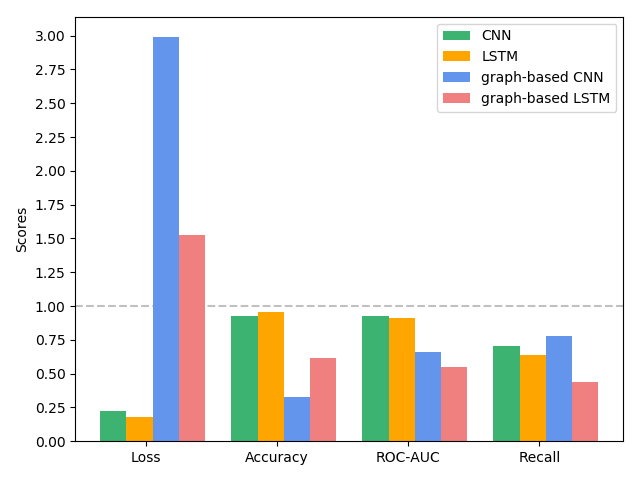
\includegraphics[width=0.7\textwidth]{pred_sequence1000_plots}
    \caption{Barplot of results of the models for the problem of prediction on a sequence with the target 1000 time steps (2 seconds) forward}
    \label{fig:pred_sequence1000_plots}
\end{figure}

For this configuration, the CNN model looked at sequences of 200 time steps each; the LSTM model looked at sequences of 500 time steps each; both the graph-based models looked at sequences of 5000 time steps each, corresponding to 10 graphs, each one representing a window of 500 time steps.

Table \ref{tab:pred_sequence2000_results} and the barplot in Figure \ref{fig:pred_sequence2000_plots} show the results for the prediction of a target 2000 time steps (4 seconds) forward with respect to the associated sequence.
\newpage
\begin{table}[htbp]
    \centering
    \begin{tabular}{lllll}
        \hline
                          & \multicolumn{4}{c}{\textbf{Metric}}                                    \\ \cline{2-5} 
        \textbf{Model}    & \textit{loss} & \textit{accuracy} & \textit{ROC-AUC} & \textit{recall} \\ \hline
        CNN               & 0.236         & 94.0 \%           & 0.911            & 0.604           \\
        LSTM              & 0.204         & 95.6 \%           & 0.932            & \textbf{0.767}  \\
        graph-based CNN   & 2.549         & 32.8 \%           & 0.642            & 0.790           \\
        graph-based LSTM  & 2.103         & 46.7 \%           & 0.475            & 0.463           \\\hline
    \end{tabular}
    \caption{Results of the models for the problem of prediction on a sequence with the target 2000 time steps (4 seconds) forward}
    \label{tab:pred_sequence2000_results}
\end{table}

\begin{figure}[htbp]
    \centering
    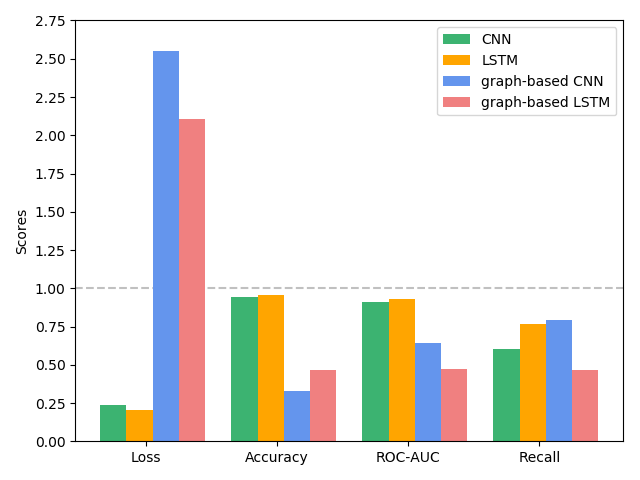
\includegraphics[width=0.7\textwidth]{pred_sequence2000_plots}
    \caption{Barplot of results of the models for the problem of prediction on a sequence with the target 2000 time steps (4 seconds) forward}
    \label{fig:pred_sequence2000_plots}
\end{figure}

For this configuration, the CNN model looked at sequences of 500 time steps each; the LSTM model looked at sequences of 500 time steps each; both the graph-based models looked at sequences of 5000 time steps each, corresponding to 10 graphs, each one representing a window of 500 time steps.

\paragraph{} As regards to the first case (\texttt{'target steps ahead'}=500) and the third case (\texttt{'target steps ahead'}=2000), the \acs{lstm} model obtained the best results, while in the second case (\texttt{'target steps ahead'}=1000) the \acs{cnn} performed better. In general, the two models were able to achieve about 0.70 of recall, which is a great result considering the extremely limited amount of data. The \acs{lstm} obtained the absolute best result with a recall equal to 0.767 for the prediction on a sequence with the target 4 seconds forward.

On the other hand, the performances of the graph-based models were unsatisfactory and very similar to the ones obtained on the task of detection on a sequence. Also in this case, the high recall reached by the graph-based \acs{cnn} is due to a prediction that is almost random, as suggested by the ROC-AUC values, and that most of the time is equal to 1, leading to a low accuracy and very high loss.


\subsection{Comments on the results}
\paragraph{} In general, the results obtained from the experiments were very respectable, given the complexity of the problem and the restricted amount of data. Based on the results, we were able to confirm some assumption, but also to reconsider other ideas.

The task of seizure detection based on a single time step confirmed our expectations: probably the information to correctly detect a seizure is partially included in the time series and not expressed only by the features of a single time step. This is confirmed also by the fact that the models obtained good results on the same task of detection, but based on a sequence. Surprisingly, the task on which the models performed better was the most difficult one, that is the seizure prediction based on a sequence. For this task, the models where able to achieve a recall higher than 0.70, which is an excellent result considering the few data used compared to previous approaches, where way more data have been used.

Overall, the model that performed better was the \acs{lstm} neural network, which most of the times obtained the highest value for recall, accuracy and ROC-AUC and the lowest value for the loss. Also the \acs{cnn} model performed very well, obtaining similar results. The models that curiously did not obtain the results expected were the graph-based \acs{cnn} and \acs{lstm} models. We tested these models with the assumption that they could outperform the standard deep learning models, since the graph representation of the brain activity is a common practice in the field of neuroscience and the application of graph-based models has recently produced good results. Unfortunately, the performances achieved by the graph-based models in this project were really poor, as we were not able to identify a good threshold between overfitting and underfitting.

There could be several reasons explaining the poor performances of the graph-based models on this type of tasks. First of all, these models were trained on graphs representing the functional connectivity between electrodes and functional connectivity networks are extremely sensitive to the choice of the connectivity metric, which in our case was the correlation coefficient. It is possible that the information that characterize the epileptic phenomenon did not arise from the configuration used to create the graphs, even if the connectivity metric has been chosen based on the literature. Another reason for the poor results obtained is the fact that graph-based models significantly suffer the lack of data. This could be a big problem for the seizure prediction task, since in a real-world scenario, seizure data are difficult to gather and we tried to reproduce a setting as real as possible by limiting the amount of available data. Therefore, this could explain why our graph-based models obtained bad performances in comparison to other studies about graph-based epileptic seizure detection which use datasets containing up to thousands of seizures (i.e. \cite{arXiv:graphseizuredet}).
